%-----------------------------------------------------------------
%Author: Yan Naing Aye
%Date:   2012 Feb 24
%-----------------------------------------------------------------
\documentclass[12pt,a4paper]{report}      % Specifies the document class
\usepackage{graphicx} %for pdf, bitmapped graphics files
\usepackage{amsmath} %to facilitate writing math formulas and to improve the typographical quality
\usepackage{amssymb}  %provides an extended symbol collection
\usepackage{wasysym} %pro­vides many glyphs
\usepackage{epstopdf} %converts eps to pdf
\usepackage{xcolor} %color extensions (for tables)
\usepackage{datetime} %date time
\usepackage[pdftitle={Aye-Thesis},pdfauthor={Yan Naing Aye}]{hyperref}
\hypersetup{
	colorlinks,
	citecolor=black,
	filecolor=black,
	linkcolor=black,
	urlcolor=black
}
\usepackage{lststyles}
%-----------------------------------------------------------------
%change to Burmese language
\usepackage{burmese}
%-----------------------------------------------------------------
%Macros
\def\titleSentence{မြန်မာဘာသာ အတွက် LaTeX Report ပုံစံ}
% I use this title in several places throughout the report
% that is why I define it as \titleSentence command 
% so that I only need to change here and all will be updated accordingly
%-----------------------------------------------------------------
%Date format
\newdateformat{mydate}{\monthname[\THEMONTH] \THEYEAR}
%-----------------------------------------------------------------
% Define a new command called \los to include list of symbol easily.
% It is used in ListOfSymbols.tex file
\newcommand{\los}[2]{\parbox[t]{5cm}{$#1 \dotfill$}  \parbox[t]{10cm}{#2}\\[0.6cm]}                                                   
%-----------------------------------------------------------------        
\renewcommand{\baselinestretch}{1.5} %linespace
%-----------------------------------------------------------------
\pagestyle{headings}    %to use headings style
%-----------------------------------------------------------------
\makeatletter
\def\input@path{{./Files/}}
\makeatother
\graphicspath{{./Fig/}}

\begin{document}        %End of preamble and beginning of text.
	\begin{titlepage}

\begin{center}
{\LARGE  \bfseries \titleSentence}\\[1cm]

% Upper part of the page   

\includegraphics[width=8cm]{XeTeX_Logo.pdf}\\[5cm]   
 
\vfill

\textsc{\large XeLaTeX ဖြင့်အသုံးပြုခြင်း}\\[1cm]

%\emph{\large နမူနာပုံစံ}\\[2cm]


{\Large \bfseries ကိုအေး}\\[1cm]

% Bottom of the page
{\large \mydate\today}

\end{center}
\end{titlepage} %Title page 
	%-----------------------------------------------------------------------------
	\newpage
	\pagenumbering{roman}  %added it if has Acknowledgment
	\begin{abstract}
		XeLaTeX ကို အသုံးပြု၍ မြန်မာ ဘာသာဖြင့် report ရေးသားရန် နမူနာ ပုံစံ ( template) တစ်ခု ဖြစ်သည်။
	\end{abstract}
	%-----------------------------------------------------------------
	\newpage
	\chapter*{ကျေးဇူးတင်လွှာ}
	\addcontentsline{toc}{chapter}{ကျေးဇူးတင်လွှာ}
	ကျွန်တော့် အပေါ် ချစ်ခင်၊ သည်းခံ၊ ဖြည့်ဆည်း ပေးသော ချစ်ဇနီး မမြ ကို ကျေးဇူးတင်ကြောင်း ပြောချင်ပါသည်။ 
	% -----------------------------------------------------------------
	\newpage
	\addcontentsline{toc}{chapter}{မာတိကာ}
	\tableofcontents
	%------------------------------------------------------------------
	\newpage
	\addcontentsline{toc}{chapter}{ပုံများ}
	\listoffigures
	%-----------------------------------------------------------------
	\newpage
	\addcontentsline{toc}{chapter}{ဇယားများ}
	\listoftables
	\clearpage
	%-----------------------------------------------------------------
	\newpage
	\markboth{သင်္ကေတများ}{သင်္ကေတများ}
	\chapter*{သင်္ကေတများ\hfill} 
	\addcontentsline{toc}{chapter}{သင်္ကေတများ}
	%List of symbols
\los{LaTeX}{Lamport TeX}
\los{XeTeX}{A TeX typesetting engine using Unicode and supporting modern font technologies.}

	\clearpage
	%-----------------------------------------------------------------
	\newpage
	\pagenumbering{arabic}
	\setcounter{page}{1}
	%-----------------------------------------------------------------
	%For code listing number
	\renewcommand{\thelstlisting}{\burmesecounter{chapter}.\burmesecounter{lstlisting}}
	%-----------------------------------------------------------------
\chapter{မိတ်ဆက်}
\label{ch:Introduction}

မြန်မာဘာသာဖြင့် ရေးသား ထားသည် များကို အသုံးပြုရန် ယူနီကုဒ်ကို ထောက်ပံ့သော XeLaTeX ကို အသုံးပြုရန် လိုသည်။ 
%------------------------------------------------------------------------------
\section{TeXstudio ကို Configure လုပ်ခြင်း}

နမူနာ အနေနှင့် အသုံးများသော LaTeX editor တစ်ခုဖြစ်သည့် TeXstudio ကိုသုံးမည်။
အောက်ပါ ဇယား~\ref{tbl_eg} တွင် အသုံးပြုထားသည့် style ဖိုင်များကို ပြထားသည်။

\begin{table}[h]\footnotesize
	\centering	
	\caption{ဖိုင်များ၏ဇယား။}
\begin{tabular}{| c | c | }	
	\hline
	ဖိုင်  & ဖော်ပြချက် \\
	\hline
	burmese.sty & မြန်မာစာ ပြောင်းပေးသည့် ဖိုင်။  \\
	\hline
	lststyles.sty & code listing များ၏ စတိုင်။  \\
	\hline
\end{tabular}
	\label{tbl_eg}
\end{table}

\section{ဖောင့်ပြင်ခြင်း}

အသုံးပြုသည့် မြန်မာဖောင့်ကို ပြင်လိုပါက burmese.sty ဖိုင်တွင် ပြင်ရမည်။
 ဥပမာ Pyidaungsu ဖောင့်သုံးလိုပါက
\begin{lstlisting}[style=myTeX,caption={မူရင်ဖောင့် သတ်မှတ်ချက်။},label={lstMTFont}]
\setmainfont{Myanmar Text}
\end{lstlisting}
 နေရာတွင်
\begin{lstlisting}[style=myTeX,caption={ဖောင့်အမည်ကိုပြင်ခြင်း။},label={lstPDFont}]
\setmainfont{Pyidaungsu}
\end{lstlisting}
 ဟုပြင်နိုင်သည်။ 

%-----------------------------------------------------------------
\chapter{ပုံစံကိုစိတ်တိုင်းကျပြုပြင်ခြင်း}
\label{ch:description}
%------------------------------------------------------------------------------
Options menu > Configure TeXstudio... ကို နှိပ်၍ General > Font တွင် IDE အတွက် မြန်မာ ဖောင့်ကို ရွေးပါ။
ထို pop-up window ၌ပင် Build > Default Compiler အတွက် XeLaTeX ကိုရွေးပါ (ပုံ~\ref{Fig_build})။
Editor > Font Family တွင် editor အတွက် မြန်မာဖောင့် ရွေးပါ။

\begin{figure*}[htbp!]
	\centering
	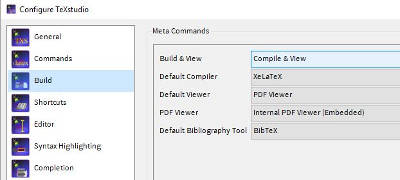
\includegraphics[width=0.8\textwidth]{build.JPG}
	\caption{Build အတွက် XeLaTeX ကို ရွေးခြင်း။}
	\label{Fig_build}
\end{figure*}



%-----------------------------------------------------------------
\chapter{နိဂုံး}
\label{ch:Conclusion}

အဓိက ရည်ရွယ်ချက် မှာ မြန်မာ ဘာသာ ဖြင့် စာတမ်း၊ သီးစစ် များ ရေးသားရာတွင် အကိုအကား နမူနာ ရယုံမျှသာ ဖြစ်သည်။ မှားယွင်းမှု၊ လိုအပ်မှုများ ရှိလျင် ကျေးဇူးပြု၍ သီးခံ၊ ဖြစ်နိုင်ပါက \href{https://github.com/yan9a}{https://github.com/yan9a} တွင် အကြောင်းကြား ပေးရန် မေတ္တာ ရပ်ခံ ပါသည် \cite{Aye201702}။


%-----------------------------------------------------------------
\appendix
\chapter{ဖြည့်စွက်ချက်}
%------------------------------------------------------------------------------
\section{မြန်မာပြန်ဆိုချက်များ}

မြန်မာပြန်ဆိုချက်များကို ပြင်လိုပါက burmese.sty ဖိုင်တွင် ဥပမာ မာတိကာ ဆိုပါက
\begin{lstlisting}[style=myTeX,caption={မြန်မာပြန်ဆိုချက်နမူနာ},label={listoflists}]
\renewcommand { \contentsname } { မာတိကာ } 
\end{lstlisting}
ဟူသည့် စာကြောင်းတွင် လိုသလို ပြင်နိုင်သည်။ 



%-----------------------------------------------------------------
\bibliographystyle{ieeetr}
\bibliography{./Files/Ref}
\addcontentsline{toc}{chapter}{အကိုးအကားများ}
% -----------------------------------------------------------------
\end{document}
% -----------------------------------------------------------------